\subsection{OSN 32 Численное решение задачи Коши для обыкновенных дифференциальных уравнений. Примеры методов Рунге-Кутта.}

% Пишет Дима

Рассматривается задача Коши для системы ОДУ:
\begin{equation}
%
    \label{Koshi_sys}
    %
    \begin{cases}
    %
        \dfrac{du}{dt} = f(t, u(t)), \quad t > 0, \\
        u(0) = u_0,
    %
    \end{cases}
    %
\end{equation}
%
где
$u(t)=\left(u_1(t), \dots, u_m(t)\right)^T$, $f(t, u(t)) = \left(f_1(t, u(t)), \dots, f_m(t,u(t)\right)^T$.

Обозначим $ | u(t) | = \sqrt{u_1^2(t) + u_2^2(t) + \ldots + u_m^2(t)}$.

\textbf{Теорема}: Пусть $f(t, u(t))$ непрерывна в параллелепипеде 
$ R = \{|t| \leqslant a, | u(t)-u(0)| \leqslant b,\; a, b\in\mathbb{R}\} $ 
и уд-ет в $R$ условию Липшица по второму аргументу, т.е. 
$|f(t, u) - f(t, v)| \leqslant L|u - v|$
, для всех $(t, u)$, $(t, v) \in R$\\ 
$\implies $
$\exists!$ решение $u(t)$ задачи \eqref{Koshi_sys}, определенное и непрерывное на некотором отрезке.


% В настоящее время наибольшее распространение получили две группы численных
% методов решения задачи Коши:
% %
% \begin{enumerate}
%     \item Методы Рунге--Кутта;
%     \item Многошаговые разностные методы, наиболее известными из которых являются
%         методы Адамса.
% \end{enumerate}

В приведенных ниже примерах для простоты изложения предполагается, что
система \eqref{Koshi_sys} состоит всего из одного уравнения.

\centerline{\textbf{Нахождение численного решения}}


Для нахождения численного решения вводится сетка по времени с постоянным шагом $\tau>0$, т.е. множество точек
$\omega_\tau = \{t_n = n\tau,\;n \in \mathbb{Z}_+\}$, и обозначим
$u_n = u(t_n)$, $f_n = f(t_n, u_n)$.
Точное решение задачи \eqref{Koshi_sys} будем обозначать буквой $u$,
а \textbf{приближенное решение} (сеточная ф-ия) --- буквой $y$: $y_n = y_n(t_n)$.

\todo{ про численное решение }

\bigbreak

\centerline{\textbf{Двухэтапный метод Рунге--Кутта}}
Общий вид двухэтапного метода Рунге--Кутта для уравнения \eqref{Koshi_sys}:
\begin{equation}
%
    \label{Runge-Kutt}
    %
    \begin{cases}
    %
        \dfrac{y_{n+1} - y_n}{\tau} = \sigma_1 K_1 + \sigma_2 K_2,~~~n\in \mathbb{Z}_+ \\
        y_0 = u_0, \\
        K_1 = f(t_n, y_n), \quad K_2 = f(t_n + a_2\tau, ~ y_n + b_{21} \tau f(t_n, y_n)),
    %
    \end{cases}
    %
%
\end{equation}
где $\sigma_1, \sigma_2,a_{2}, b_{21} \in\mathbb{R}$~"--- некоторые числа, от выбора которых зависит как погрешность аппроксимации, так и точность численного решения.

Подставим значения $K_1$ и $K_2$ в первое уравнение системы \eqref{Runge-Kutt}:
%
$$
    \frac{y_{n+1} - y_n}{\tau} = \sigma_1 f(t_n, y_n) +
    \sigma_2 f(t_n + a_2 \tau, y_n + b_{21} \tau f(t_n, y_n)).
$$
%
Рассмотрим \textbf{погрешность аппроксимации} разностной схемы \eqref{Runge-Kutt}
на решении задачи \eqref{Koshi_sys}:
%
\begin{equation}
%
    \label{Runge-Kutt_appr}
    %
    \psi_n = - \frac{u_{n+1} - u_n}{\tau} + \sigma_1 f(t_n, u_n) +
    \sigma_2 f\left(t_n+a_2\tau, u_n + b_{21}\tau f(t_n, u_n)\right).
%
\end{equation}

\textbf{Утв.}: Погрешность аппроксимации этого метода имеет второй порядок малости по $\tau$: $\psi_n = O(\tau^2)$ при $\sigma_2 = \sigma, \sigma_1 = 1-\sigma, a_2 = b_{21} = \sigma/2$.

\begin{proof}

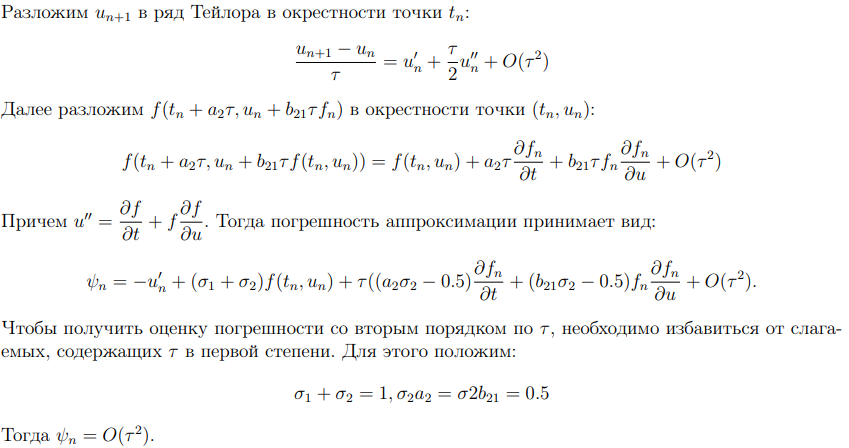
\includegraphics[scale=0.4]{pics/osn_31_new.png}

\end{proof}

\textbf{Погрешность решения} разностной схемы~\eqref{Runge-Kutt}: $z_n = y_n - u_n,  n\in\mathbb{Z}.$

\textbf{Утв.}: Общий двухэтапный метод Рунге--Кутта
при выполнении соответствующих условий
имеет квадратичную точность по $\tau$, т.е. при достаточно малых $\tau$: $|z_{n+1}| = O(\tau^2)$, совпадающую с оценкой погрешности аппроксимации на решении исходного уравнения \eqref{Koshi_sys}

Частные случаи общего двухэтапного метода Рунге--Кутта:

\begin{enumerate}
%
    \item При $\sigma=1,~~a=a_2=0.5,~~b=b_{21}=0.5$ мы получим схему Рунге--Кутта <<предиктор--корректор>>:
    $y_{n+1} = y_n + \tau f(t_{n+\frac12}, y_n + 0.5\tau f(t_n, y_n)).$
    Погрешность этой схемы равна $O(\tau^2)$.

    \item Если положить $\sigma=0.5,~~a=1,~~b=1$, то мы получим симметричную разностную схему:
    %
    $$\dfrac{y_{n+1} - y_n}{\tau} = 0.5 \left(f(t_n, y_n) +
      f(t_n + \tau, y_n + \tau f_n)\right), n\in\mathbb{Z}_+, y_0 = u_0.
    $$
    %
    Эта разностная схема является очень эффективной, имеет второй
    порядок точности по $\tau$ и часто используется на практике.
    %
\end{enumerate}




\centerline{\textbf{Общий $m$-этапный метод Рунге--Кутта}}

Общая идея $m$-этапного метода Рунге--Кутта заключается в том, что
для вычисления значения приближенного решения в каждой следующей точке $t_{n+1}$
вводятся $m$ дополнительных этапов.
Промежуточные значения на каждом шаге $n\in\mathbb{Z}_+$ вычисляются по формулам:
$$
\begin{aligned}
%
    &K_1 = f(t_n, y_n), \\
    &K_2 = f(t_n + a_2\tau, y_n + b_{21} \tau K_1), \\
    &K_3 = f(t_n + a_3\tau, y_n + b_{31}\tau K_1 + b_{32}\tau K_2), \\
    &\dots \\
    &K_m = f(t_n+a_m\tau, y_n + b_{m1} \tau K_1 + b_{m2} \tau K_2 + \ldots + b_{m m -1} \tau K_{m-1}).
%
\end{aligned}
$$
%
При этом разностная схема для исходной задачи~\eqref{Koshi_sys}
имеет вид
%
\begin{equation}
    %
    \label{gen_Runge-Kutt_meth}
    %
    \begin{cases}
        \dfrac{y_{n+1} - y_n}{\tau} = \sigma_1 K_1 + \sigma_2 K_2 + \ldots + \sigma_m K_m \\
        y_0 = u_0, n \in \mathbb{Z}_+,
    \end{cases}
    %
\end{equation}
%
где $\sigma_1, \ldots, \sigma_m \in\mathbb{R}$, и выполнено условие аппроксимации: $\sum\limits_{i=1}^{m} \sigma_i = 1.$

Примеры трех- и четырех- этапных методов Рунге--Кутта, имеющих третий и четвертый порядок точности соответственно:
%

\begin{enumerate}
%
    \item \textbf{$m=3$}: $\dfrac{y_{n+1} - y_n}{\tau} = \frac16(K_1 + 4K_2 + K_3),$ где
    %
    $$
        \begin{aligned}
            &K_1 = f(t_n, y_n), \\
            &K_2 = f(t_n + 0.5 \tau, y_n + 0.5 \tau K_1), \\
            &K_3 = f(t_n + \tau, y_n - \tau K_1 + 2\tau K_2).
        \end{aligned}
    $$
    Данная схема имеет третий порядок точности по $\tau$: $O(\tau^3)$.

    \item \textbf{$m=4$}: $\dfrac{y_{n+1} - y_n}{\tau} = \frac16 (K_1 + 2K_2 + 2K_3 + K_4),$ где
    
    $$
        \begin{aligned}
            &K_1 = f(t_n, y_n), \\
            &K_2 = f(t_n+0.5\tau, y_n + 0.5\tau K_1), \\
            &K_3 = f(t_n + 0.5 \tau, y_n + 0.5 \tau K_2), \\
            &K_4 = f(t_n + \tau, y_n + \tau K_3).
        \end{aligned}
    $$
    Данная схема имеет четвертый порядок точности по $\tau$: $O(\tau^4)$.

\end{enumerate}

%
\textbf{Замечание}: Формулы $m$-этапного метода Рунге--Кутта достаточно громоздки. Это является одной из причин того, что на практике редко используются методы Рунге--Кутта для $m > 4$.
%




% -------- source --------
\bigbreak
[\cite[page 152-163]{chimi}]